\documentclass{article}
\usepackage{a4wide}
\usepackage[latin1]{inputenc}
\usepackage{epsfig}
\usepackage{graphicx}
\usepackage{subcaption}
\usepackage{mathtools}

\sloppy

\begin{document}
	
	% Titelseite ---------------
		\title{The Scale-Invariant-Feature-Transform} 
		\author{Leopold Gaube}
		\date{15.01.2017} 
		\maketitle
		
	\begin{abstract}
		
	(...Computers no longer only understand their own world of numbers and maths. Nowadays some computer algorithmns are good enough to cope with our human world. accurately detect, track and recognize objects in still or moving images. )
	
	The following paper is supposed to give an overview of how the Scale-Invariant Feature Transform, short SIFT, works. It was introduced by David G. Lowe in 1999 and enhanced multiple times until he published his final version in 2004. This algorithm extracts distinctive features which can be used for matching objects acorss multiple images.
	
	\end{abstract}
	
	
	
	\section{Introduction}
	\subsection{Motivation and Usage}
	
	The main goal of the Scale Invariant Feature Transform is finding distinct points in an image which are likely to appear in a different image, depicting the same object(s). These distinct points are called keypoints and are being used to compute a feature descriptor which summarizes the local neighbourhood around that keypoint's location. 
	
	Supposing that corresponding keypoints can be found over multiple images, ... correct matches of their feature descriptors can in turn be used in a range of computer vision tasks. 
	
	Lowe proposed a way of how SIFT features can be used to recognize objects even under difficult conditions. A Hough-transform is being used to even detect object which are partially occluded. Furthermore SIFT can also be used for tracking objects in videos.
		
	...Gesture recognition to control applications or tell robots what to do.
	
	In 2007 Lowe collaborated with Matthew Brown to published a paper on how to
	use these invariant features to stitch partially overlaping images together into a single panoramic image. ["Automatic Panoramic Image Stitching using Invariant Features"]
	
	\section{Extracting SIFT Features}		
	\subsection{Selecting keypoints from scale-space extrema}
	
	The first step of the SIFT algorithm is to extract potential keypoints.
	It would be a bad idea for an image feature-based algorithm to consider every possible pixel location, because computation for a single image would take a long time and most features would be unusable for exact localization due to their lack of image information. 
	
	That is why a (sampling strategy) has to be applied in order to find good keypoints. A keypoint is considered good, if its feature exhibits a (high recognition value). Therefore, it should be invariant to numerous transformations such as rotation, scale, distortion and brightness but also to change in illumination, 3D viewpoint and addition of noise. Of course, it would be really hard to satisfy all those properties, but the Scale-Invariant-Feature-Transform turns out to be quite good, which will further be examined in this paper.
	
	Lowe uses for his keypoint sampling approach a so-called scale-space representation of the given image. That means the image will be smoothed with different scales $\sigma$ of the Gaussian blur(/kernel). Smoothing/Blurring (synonym?) an image with a low $\sigma$ value will suppress fine structures, whereas smoothing with a large $\sigma$ only leaves coarse/rough contours. The results of the Gaussian blurring can be seen in figure 1(b) and 1(c). That is exactly what we need in order to find distinctive features no matter how large or small they are depicted in the image. The resulting images stack-up to form a Gaussian pyramid.
	
	Lowe has found that using an initial $\sigma = 1.6$ and gradually adjusting each ensuing scale of the Gaussian blur by a constant factor of $k = 2^{1/3}$ will achieve the best results [reference paper].
	
	After every three blurred images - which also means after each doubling of the $\sigma$ scale - the image can be downsampled by a factor of two. All images of the same size in the pyramid are considered to form an octave. The accuracy of sampling relative to $\sigma$ stays roughly the same for all octaves, but results in major computational performance boosts.
	
	Subtracting one Gaussian blurred image pixelwise from another results in a Difference of Gaussians. Doing this for every two neighbored images of the same octave in the Gaussians pyramid gives us a Difference of Gaussians (DoG) pyramid with one image less in each octave then before. In order to compensate for this lost image, we previously need to compute one more Gaussian blurred image at the end of each octave. Keep in mind that the resampling for the first image of the next octave should to be done on the same image as before.
	
	To finally retrieve the potential keypoints, each pixel of every Difference of Gaussian (except the first and last of each octave --> reason + 2 more Gaussian images needed!!!) is compared to its eight pixel neighbors as well as its 18 neighbors from the DoGs laying directly above and below it in the pyramid (see figure 2.x). A pixel's location is taken into the set of our potential keypoints only if its value is either a minimum or a maximum in its surrounding neighborhood. 
	
	As mentioned before smoothing/blurring an image with different strengths results in images with a different amount of detail. A minimum or maximum in scale-space means that a structure is still visible in one Gaussian image, but has been "smoothed away" by the stronger Gaussian kernel of the next. This leads to a large pixel value difference along the structure between these two Gaussians. A Difference of Gaussians has therefore a strong response to edges, as explicated in "Gaussian-based edge-detection methods-a survey" by M. Basu.

	(-->lenna DoG)
	
	If we look at two images depicting the same object, but one taken from further away, we will still find corresponding keypoints, but on different scales of the DoG pyramid. --> Scale Invariant
	
	\begin{figure}[ht]
		\begin{center}
			\begin{subfigure}[normla]{0.3\textwidth}
				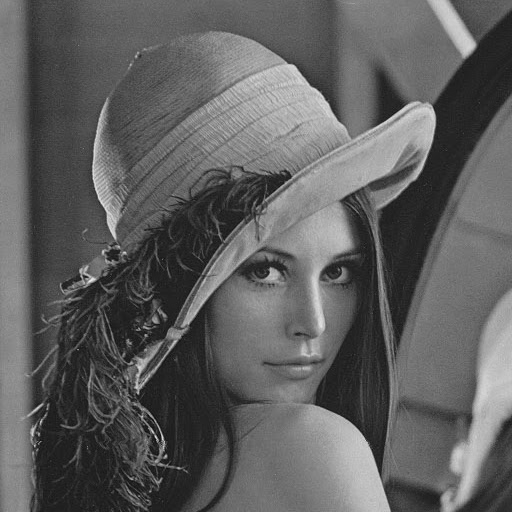
\includegraphics[width=4.5cm]{images/lenna.png}
				\caption{Original image}
				\label{subfig:org}
			\end{subfigure}
			~
			\begin{subfigure}[normla]{0.3\textwidth}
				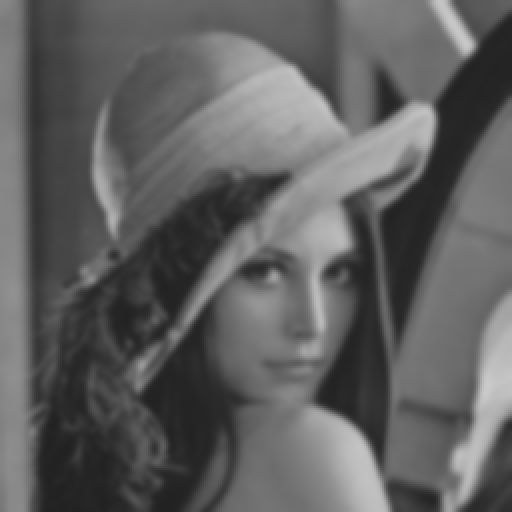
\includegraphics[width=4.5cm]{images/gaussian_at_sigma_3.png}
				\caption{Gaussian with $\sigma = 1.6$}
				\label{subfig:gauss1}
			\end{subfigure}
			~
			\begin{subfigure}[normla]{0.3\textwidth}
				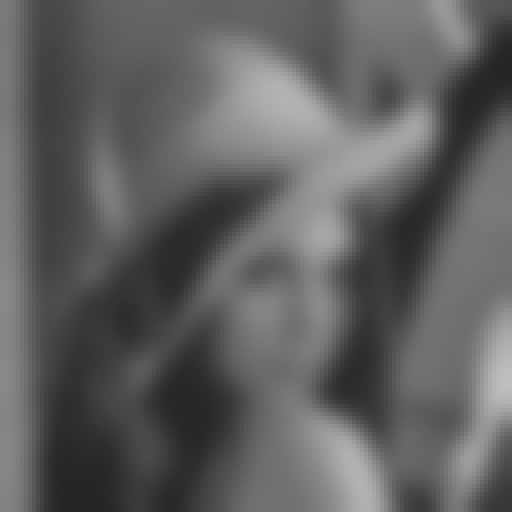
\includegraphics[width=4.5cm]{images/gaussian_at_sigma_10.png}
				\caption{Gaussian with $\sigma = ?$}
				\label{subfig:gauss2}
			\end{subfigure}
		
			\vspace{0.3cm}
		
			\begin{subfigure}[normla]{0.3\textwidth}
				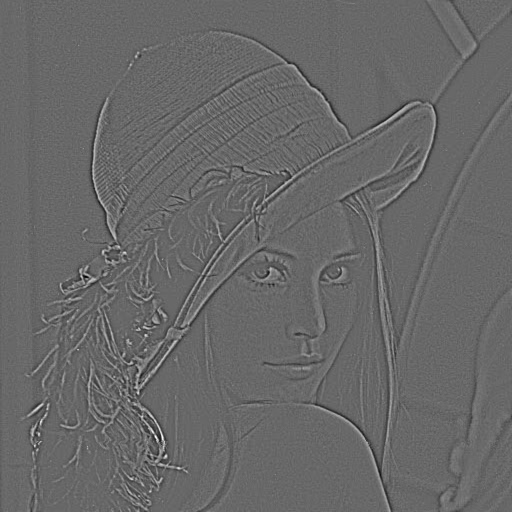
\includegraphics[width=4.5cm]{images/DoG_at_sigma_2.png}
				\caption{DoG with $\sigma_1$=1.6, $\sigma_2$=2.0}
				\label{subfig:org}
			\end{subfigure}
			~
			\begin{subfigure}[normla]{0.3\textwidth}
				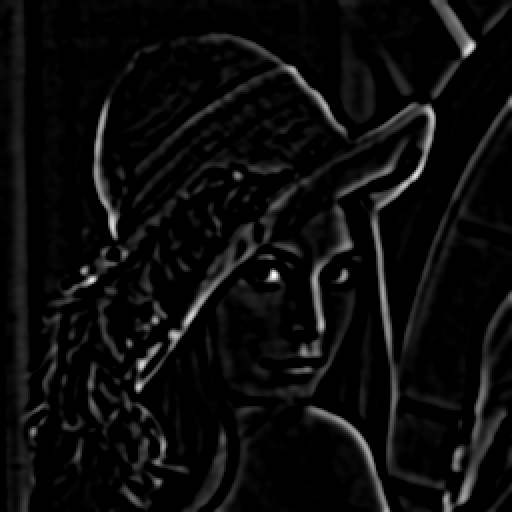
\includegraphics[width=4.5cm]{images/DoG_at_sigma_5.png}
				\caption{DoG with $\sigma_1$=?, $\sigma_2$=?}
				\label{subfig:org}
			\end{subfigure}
			~
			\begin{subfigure}[normla]{0.3\textwidth}		
				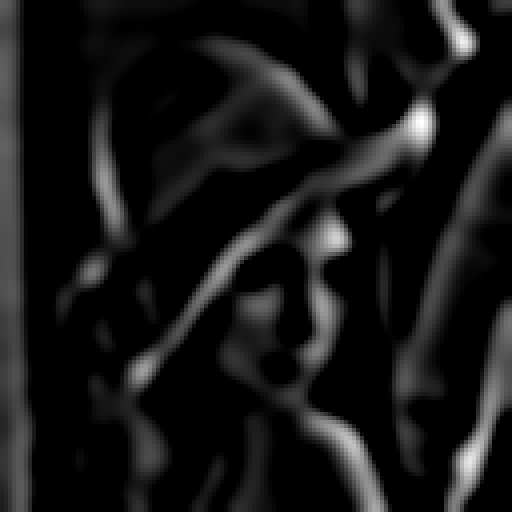
\includegraphics[width=4.5cm]{images/DoG_at_sigma_13.png}
				\caption{DoG with $\sigma_1$=?, $\sigma_2$=?}
				\label{subfig:org}
			\end{subfigure}
		\caption{This figure shows the impact of the Gaussian blur with different scales $\sigma$ on an image as well as the normalized difference of two neighboured Gaussian images.}
		\end{center}
	\end{figure}
	
	\subsection{Keypoint refinement}
	
	Our next step in the SIFT algoritthm is to precisely predict the location and scale of the keypoints by on a subpixel precision level. It is done by fitting a quadratic surface to the sample points which we have chosen from the scale space extrema.
	
	
	\subsection{Keypoint filtering}
	
	Some of the keypoints we obtained earlier might not serve for good features due to a lack of contrast or unstable localization along an edge, so we need to reject such keypoints. 
	A low contrast also means that we might not find corresponding features of the same object in an image that has slightly been transformed from the original. The contrast  can easily be computed by the tayler expansion of the scale space function shifted by the exact location of the extremum. 
	
	$$
	D(\hat x) = D + \frac{1} {2} \frac{\partial D^T} {\partial x} \hat x
	$$
	
	Lowe found that if the absolute value of that function is less than 0.03 there is just not enough contrast for it to be a stable feature. (normalized pixel values [0..1])
	
	Even if there is enough contrast the algorithm might still struggle to exactly localize a keypoint along an edge. That is why we rather have corner-like features than only edge-like.
	
	To further illustrate this problem, we can simply look at an arbitrary thick white line on black background as shown in Figure 3(a). If we were to cut a patch from the middle section of the line 3(b), it would be impossible to tell at which exact location on the line the patch originated from. A patch of one of the end sections 3(c) can easily be matched its correct location at the corresponding end of the line.
	
	In order to mathematically determine whether a given feature is corner-like (/stable) or not, we can use a 2x2 Hessian matrix at its keypoint location and scale 
	
	\begin{figure}
		\begin{center}
			\begin{subfigure}[normla]{0.3\textwidth}
				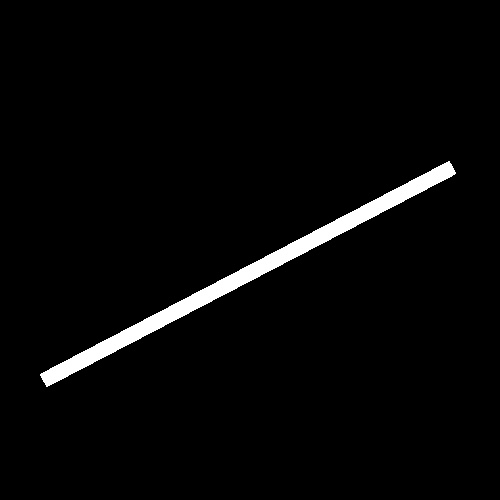
\includegraphics[width=4.5cm]{images/straight_line.png}
				\caption{Gaussian with $\sigma = ?$}
				\label{subfig:gauss2}
			\end{subfigure}
			~
			\begin{subfigure}[normla]{0.3\textwidth}
				
\includegraphics[width=4.5cm]{images/line_patch.png}
				\caption{Original image}
				\label{subfig:org}
			\end{subfigure}
			~
			\begin{subfigure}[normla]{0.3\textwidth}
				
\includegraphics[width=4.5cm]{images/corner_patch.png}
				\caption{Gaussian with $\sigma = 1.6$}
				\label{subfig:gauss1}
			\end{subfigure}	
		\end{center}
	\end{figure}
	
	\subsection{Orientation assignment}
	
	We have already shown that SIFT-Features are invariant to scale, but rotational invariance is just as important for numerus image processing tasks. For this purpose, Lowe assigns each keypoint one or more consistent orientations, based on its neighborhood's gradients.	An image gradient indicates a change of pixel intensity in a specific direction. 
	
	The most prominent gradient direction of a keypoint seems to be a good pick for assignment of a consistent orientation, because rotating an image by an angle $\phi$ will only shift all gradients by $\phi$ as well; thus, maintaining the same relative directions.
	
	To find the most prominent gradient direction, we first need to compute all gradients around a keypoint and organize them in a histogram. A histogram shows the distributing of numerical data by dividing the data in disjoint categories, called bins. In our application we will habve 36 bins and each bin represents a range of 10� out of all 360� possible angle directions. 
	
	For every Gaussian blurred image, L, all gradient directions and magnitudes are precomputed for performance purposes.
	The direction of a gradient at a certain location in L can be calculated with the following formular using pixel differences:
	$$
		\theta(x, y) = \tan^{-1}{((L(x, y + 1) - L(x, y - 1)) / (L(x + 1, y) - L(x - 1, y)))}
	$$
	The gradient's magnitude shows how strong the pixel intensity changes in the gradient's direction. It can be calculated in a similar manner:
	$$
	m(x, y) = \sqrt{(L(x + 1, y) - L(x - 1, y))^2 + (L(x, y + 1) - L(x, y - 1))^2}
	$$
	
	The magnitude of each gradient is weighted by a Gaussian function, so that gradients closer to the center of the keypoint have a higher impact than gradients further away which tend to be more unstable to minor transformations. This weighted input will be added to the bin which represents the gradient's direction. The highest peak in that histogram is the direction we are looking for. Any other peaks that holds a value higher than 80\% of the highest peak leads to the creation of an additional keypoint at the same location, but with a different orientation. These keypoints with multiple strong gradient directions are scarce, but help to make matching more stable. 
	
	A parabola is fit to the three closest values of each peak to achieve a more accurate orientation at the real maximum of that peak.
	
	(Picking up the patch matching problem of a straight line from earlier (Figure 3). Both end patches would generate similar descriptors after they have been assigned an orientation, thus matching their keyypoints could proof problematic)
	
	\subsection{Constructing the feature descriptor}
	
	There are many possibilities to describe the area around a keypoint. For instance we could be storing the intensity or color values inside our feature descriptor. However, the disadvantage of this approach is that many images are taken under different lighting conditions. Hence intensity values of corresponding keypoints might vary a lot. Image gradients are a better choice for constructing a feature descriptor, because they only coincide with change of pixel intensity rather than intensity values itself. 
	
	relative gradient directions / rotated 16x16 neighbourhood
	The SIFT feature descriptor uses gradients in a 16x16 neighbourhood around each keypoint. These gradients will further be organized in 4x4 cells, so there will be a total of 16 of those cells. Analogous to section 2.4 each cell accumulates its (magnitude and gaussian function weighted) gradients in an orientation histogram with only 8 different bins. Hence each bin represents 45� which allows for more "wiggle" room of the gradients directions...
	
	\section{Problems}
		% What SIFT cannot do!!!
	
	SIFT features can be computed relatively fast, however matching over a vast database might still take a long time. Herbert Bay addresses this problem in his publication "Speeded Up Robust Features" (SURF) from 2006. His SURF features are based on SIFT and can be computed even faster. Their smaller 64 dimensional descriptor allows for faster matching of its features with only minor loss in accuracy and are therefore better suited for (real-time applications).
	
	In one picture a subject might be well lit by sunshine and therefore have high pixel values and also strong contrast due to shadows, whereas another picture might be taken in cloud weather, resulting in low intensity values and a more flat contrast.
	
	repetative structures like a fence (Bilder) / multiple occurences of the same thing
	
	problem with outliers , RANSAC solves
	
	Robustness only to a certain point
	
	\section{Conclusion}
	
	SIFT features are a great way to corretly match many corresponding keypoints across images. Their invariance and robustness properties allow for enough laditude in change of perspective and illumination (which can never be fully avoided in images).
	
	...
	
	
\end{document}
